\subsection{Terzaghi consolidation: Two-phase}
\subsubsection*{Definition}
For this comparison, we may utilize the same analytical solution as was done for the single phase case in the previous section, although the solution must represent the mean fluid pressure $\bar{p}=S_wp_w + S_{nw}p_{nw}$, for the final relationship,

\begin{equation}
\frac{\bar{p}\left( z,t \right)}{\bar{p}_0}=\left\{ 1.0-{{\left( \frac{L-z}{L} \right)}^{2}}-\frac{32}{{{\pi }^{3}}}\left[ \sum\limits_{m=0}^{\infty }{\frac{{{\left( -1 \right)}^{m}}}{{{\left( 2m+1 \right)}^{3}}}\exp \left[ -{{\psi }^{2}}ct \right]\cos \left[ \psi \left( L-z \right) \right]} \right] \right\},
\end{equation} 

with pressure generation defined in the same manner,

\begin{equation}
{{\bar{p}}_{0}}=\frac{{{L}^{2}}}{2c}\left( {{B}_{v}}{{{\dot{\sigma }}}_{z}} \right),
\end{equation}

but where the uniaxial Skempton coefficient, ${B}_{v}$, must be defined (see Table \ref{terz:tab1}) based upon the effective fluid modulus. Fluid properties are then defined for two separate fluids (Table \ref{terz:tab4})

\begin{table}[!t]
\begin{center}
\begin{tabular}{lccc}
\hline\noalign{\smallskip}
Property & Symbol & Unit & Value \\
\noalign{\smallskip}\hline\noalign{\smallskip}
\textit{Wetting fluid properties} &          &        & \\
Bulk modulus   & $K_{w}$       & $GPa$       & $2.933$ \\
Density        & $\rho _{w} $  & $kg/m^3$    & $997.05$ \\
Viscosity      & $\mu _{w} $   & $Pa\dot s$  & $8.9008\times 10^{-4}$ \\
Saturation     & $S_{w}$       & $-$         & $0.8$ \\
\\
\textit{Non-wetting fluid properties} &               &               &  \\
Bulk modulus   & $K_{nw}$        & $GPa$       & $1.187$ \\
Density        & $\rho _{nw} $   & $kg/m^3$    & $997.05$ \\
Viscosity      & $\mu _{nw} $    & $Pa\dot s$  & $8.9008\times 10^{-4}$ \\
Saturation     & $S_{nw}$        & $-$         & $0.2$ \\
\noalign{\smallskip}\hline
\end{tabular}
\end{center}
\caption{Two-phase fluid properties.}
\label{terz:tab4}
\end{table}

\begin{figure}[!tbh]
\begin{center}
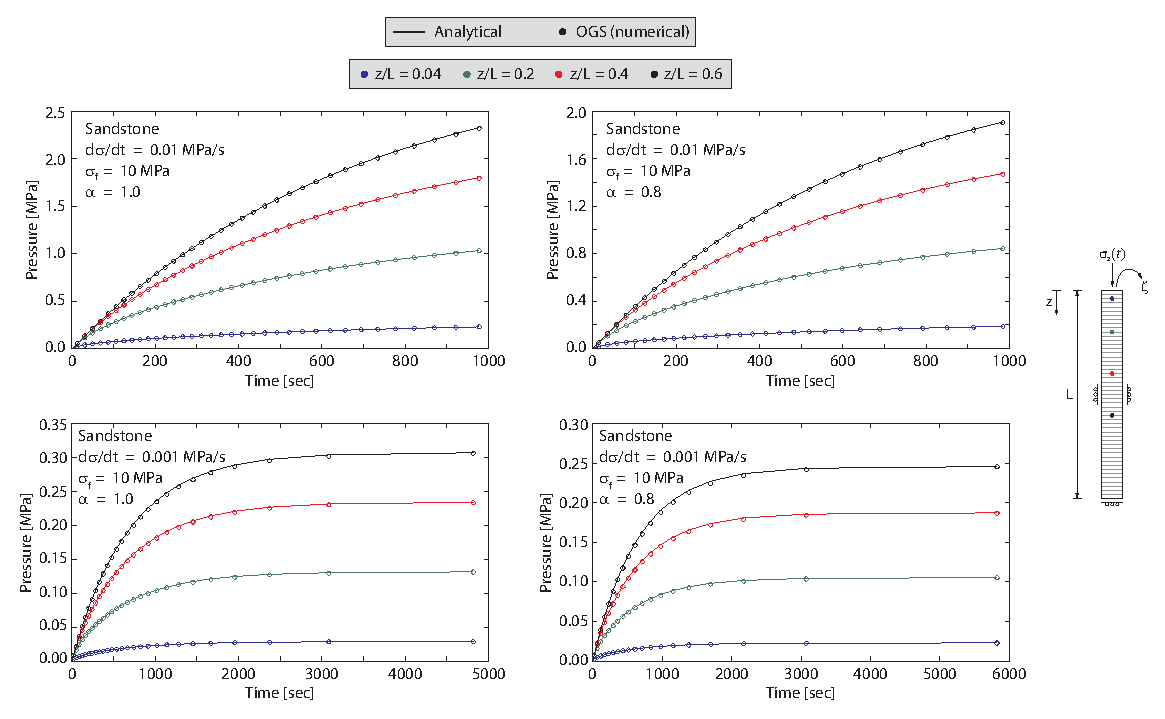
\includegraphics[width=1.0\textwidth]{chapter_14/figures/fig_14_3_21}
\end{center}
\caption{Sandstone solutions.}
\label{terz:h2msand}
%\end{figure}
%\begin{figure}[!tbh]
\begin{center}
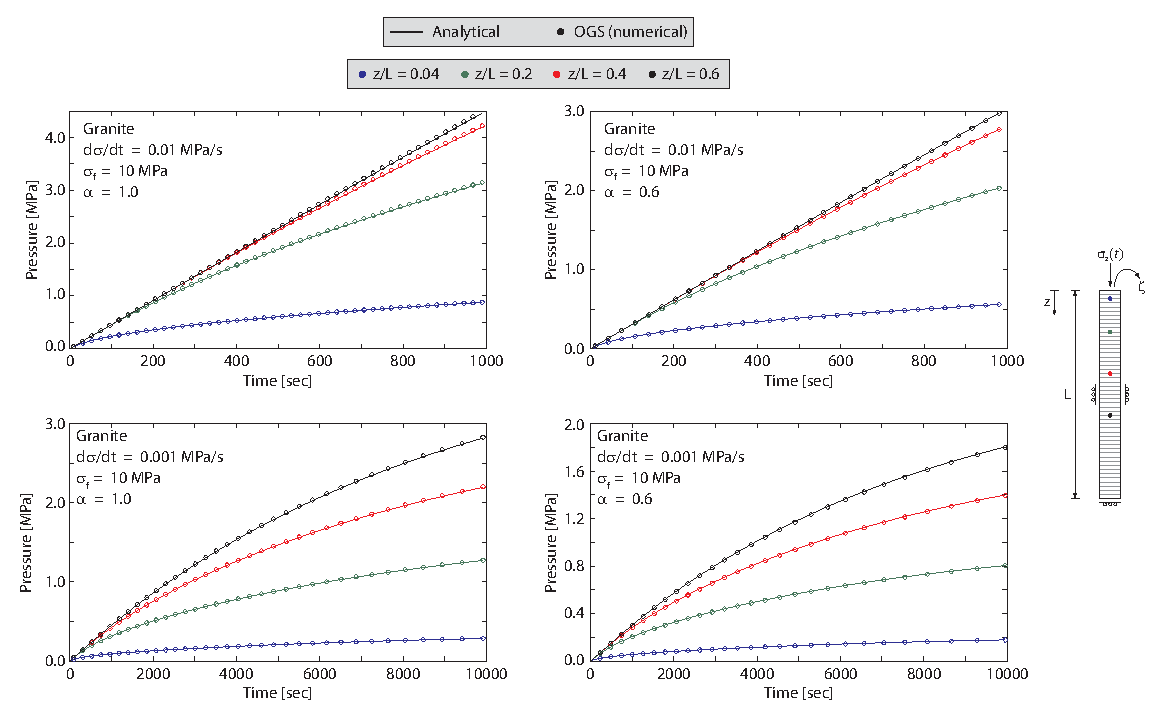
\includegraphics[width=1.0\textwidth]{chapter_14/figures/fig_14_3_22}
\end{center}
\caption{Granite solutions. Here, a porosity of 0.06 is used to ensure stability for the incompressible grain simulations (an adjustment that is not needed for compressible grains, but is used there also to maintain consistency).}
\label{terz:h2mgranite}
\end{figure}

\subsubsection*{Results}
Initially the column is at zero pressure and is saturated uniformly with both fluids ($Sw=0.8$) and we apply $p_c=0$ and $k^{r}_{w}=k^{r}_{nw}=0.5$. Note that we utilize a different compressibility for each fluid in order to exercise both fluid balance equations, with the analytical solution obtained using the \textit{effective} fluid modulus, and with the \textit{effective} modulus having an identical value to the single fluid modulus, $2.27 GPa$, used above in the single phase case.

Results are shown in Figs. \ref{terz:h2msand} and \ref{terz:h2mgranite} for sandstone and granite (see Table \ref{terz:tab2}) for incompressible and compressible grains. With reference to the staggered stability criterion discussed in the HM problem above, because we are examining incompressible grains here the solution becomes unstable for granite. Therefore, an alternate value of porosity (0.06) is utilized (in the granite simulations) to ensure stability, which results in $B_v<0.5$. Such an adjustment is not required when compressible (real) grains are used, but is utilized none-the-less for comparison with the incompressible grain solution. All results are ideally accurate. 

Time steps are adaptively controlled with a tolerance based on the rate of pressure change over a time step. Such a scheme is capable of ensuring accuracy in HM or H2M problems. Note the importance of the tolerance in Fig. \ref{terz:res1}.
